\documentclass[a4paper,14pt]{extarticle}

\usepackage[utf8x]{inputenc}
\usepackage[T1,T2A]{fontenc}
\usepackage[russian]{babel}
\usepackage{hyperref}
\usepackage{indentfirst}
\usepackage{here}
\usepackage{array}
\usepackage{graphicx}
\usepackage{caption}
\usepackage{subcaption}
\usepackage{chngcntr}
\usepackage{amsmath}
\usepackage{amssymb}
\usepackage{amsthm}
\usepackage{pgfplots}
\usepackage{pgfplotstable}
\usepackage[left=2cm,right=2cm,top=2cm,bottom=2cm,bindingoffset=0cm]{geometry}
\usepackage{multicol}
\usepackage{askmaps}
\usepackage{titlesec}
\usepackage{listings}
\usepackage{color}
\usepackage{enumerate}
\usepackage{hhline}
\usepackage{enumitem}
\usepackage{courier}
\usepackage{wrapfig}
\usetikzlibrary{arrows,automata}

\setitemize{itemsep=0em}
\setenumerate{itemsep=0em}

\theoremstyle{definition}

\pgfkeys{/pgf/number format/.cd,1000 sep={\,}}

\definecolor{green}{rgb}{0,0.6,0}
\definecolor{gray}{rgb}{0.5,0.5,0.5}
\definecolor{purple}{rgb}{0.58,0,0.82}

\lstset{
	language=python,
	backgroundcolor=\color{white},   
	commentstyle=\color{green},
	keywordstyle=\color{blue},
	numberstyle=\tiny\color{gray},
	stringstyle=\color{purple},
	basicstyle=\footnotesize\ttfamily,
	breakatwhitespace=false,
	breaklines=true,
	captionpos=b,
	keepspaces=true,
	numbers=left,
	numbersep=5pt,
	showspaces=false,
	showstringspaces=false,
	showtabs=false,
	tabsize=2,
	frame=single,
	inputpath={../code/}
}

\renewcommand{\le}{\ensuremath{\leqslant}}
\renewcommand{\leq}{\ensuremath{\leqslant}}
\renewcommand{\ge}{\ensuremath{\geqslant}}
\renewcommand{\geq}{\ensuremath{\geqslant}}
\renewcommand{\epsilon}{\ensuremath{\varepsilon}}
\renewcommand{\phi}{\ensuremath{\varphi}}
\renewcommand{\thefigure}{\arabic{figure}} 	
\newcommand{\norm}[1]{\left\lVert#1\right\rVert}
\newcommand*\sfrac[2]{{}^{#1}\!/_{#2}}

%\titleformat*{\section}{\large\bfseries} 
\titleformat*{\subsection}{\normalsize\bfseries} 
\titleformat*{\subsubsection}{\normalsize\bfseries} 
\titleformat*{\paragraph}{\normalsize\bfseries} 
\titleformat*{\subparagraph}{\normalsize\bfseries} 

\counterwithin{figure}{section}
\counterwithin{equation}{section}
\counterwithin{table}{section}
\newcommand{\sign}[1][5cm]{\makebox[#1]{\hrulefill}}
\graphicspath{{../pics/}}
\captionsetup{justification=centering,margin=1cm}
\setlength\parindent{5ex}
\def\arraystretch{1.3}
\def\tabcolsep{12pt}
%\titlelabel{\thetitle.\quad}

\DeclareMathOperator*{\argmin}{argmin}
\DeclareMathOperator*{\argmax}{argmax}

\begin{document}

\begin{titlepage}
\begin{center}
	\textbf{Санкт-Петербургский Политехнический Университет \\Петра Великого}\\[0.3cm]
	\small Институт компьютерных наук и технологий \\[0.3cm]
	\small Кафедра компьютерных систем и программных технологий\\[4cm]
	
	\textbf{ОТЧЕТ}\\ \textbf{по расчетному заданию}\\[0.5cm]
	\textbf{<<Построение моделей>>}\\[0.1cm]
	\textbf{Системный анализ и принятие решений}\\[8.0cm]
\end{center}

\begin{flushright}
	\begin{minipage}{0.4\textwidth}
		\begin{flushleft}
			\small \textbf{Работу выполнил студент}\\[3mm]
			\small группа 33501/4 \hspace*{6mm} Дьячков В.В.\\[5mm]
			
			\small \textbf{Преподаватель}\\[5mm]
		 	\small \sign[3cm] \hspace*{5mm} Сабонис С.С.\\[0.5cm]
		\end{flushleft}
	\end{minipage}
\end{flushright}

\vfill

\begin{center}
	\small Санкт-Петербург\\
	\small \the\year
\end{center}
\end{titlepage}

\addtocounter{page}{1}

\tableofcontents
%\newpage
\listoffigures
\listoftables
\newpage

\section{Техническое задание}

\begin{enumerate}
	\item Решить задачу методом Лагранжа при заданном ограничении;
	\item Решить задачу методом Била при заданных ограничениях;
	\item Решить задачу методом проекции градиента при заданных ограничениях;
	\item Решить задачу методом штрафных функций или методом барьерных функций при
заданном ограничении;
	\item Решить задачу методом возможных направлений при заданном ограничении.
\end{enumerate}

\section{Исходные данные}

\paragraph{Вариант 32}

Дана задача нелинейного программирования:
\begin{equation*}
	\max f(X) = \max \left( -31 x_1^2 - 34 x_2^2 + 4 x_1 x_2 + 286 x_1 + 388 x_2 \right)
\end{equation*}
Заданы коэффициенты $a_{ij}$:
\begin{center}
\begin{multicols}{5}
	$a_{11} = 7$\\
	$a_{21} = 10$\\
	$a_{31} = -1$\\
	$a_{41} = 0$\\
	$a_{51} = 0$\\
\end{multicols}
\begin{multicols}{5}
	$a_{12} = 12$\\
	$a_{22} = 8$\\
	$a_{32} = 0$\\
	$a_{42} = -1$\\
	$a_{52} = 1$\\
\end{multicols}
\end{center}
Заданы коэффициенты $b_i$:
\begin{multicols}{6}
	\centering
	$b_1 = 84$\\
	$b_2 = 80$\\
	$b_3 = 0$\\
	$b_4 = 0$\\
	$b_5 = 5$\\
	$b_6 = 400$\\
\end{multicols}
\noindent Заданы коэффициенты $d_i$:
\begin{multicols}{2}
	\centering
	$d_1 = 16$\\
	$d_2 = 25$\\
\end{multicols}

\section{Решение методом Лагранжа}

Решим задачу при ограничении:
\begin{equation*}
	a_{51} x_1 + a_{52} x_2 = b_5 
\Longleftrightarrow
	x_2 = 5
\Longleftrightarrow
	x_2 - 5 = 0
\end{equation*}

В методе Лагранжа исходная задача условной оптимизации сводится к задаче безусловной оптимизации -- задаче поиска стационарной точки функции Лагранжа, являющийся точкой локального максимума функции $L(X, V)$ по аргументу $X$. Запишем функцию Лагранжа:
\begin{equation*}
	L(X, V) = -31 x_1^2 - 34 x_2^2 + 4 x_1 x_2 + 286 x_1 + 388 x_2 + V_1 \left(x_2 - 5\right)
\end{equation*}

Сформулируем условие стационарности:
\begin{equation*}
\begin{cases}
	\dfrac{\partial L}{\partial x_1} = -62 x_1 + 4 x_2 + 286 = 0 \\[0.3cm]
	\dfrac{\partial L}{\partial x_2} = -68 x_2 + 4 x_1 + 388 + V_1 = 0 \\[0.3cm]
	\dfrac{\partial L}{\partial V_1} = x_2 - 5 = 0
\end{cases}
\end{equation*}

Решая систему уравнений получим:
\begin{equation*}
\begin{cases}
	x_2 = 5 \\
	-62 x_1 + 20 + 286 = 0 \\
	-340 + 4 x_1 + 388 + V_1 = 0
\end{cases}
\Rightarrow
\begin{cases}
	x_2 = 5 \\
	x_1 \approx \dfrac{286}{62} \approx 4.94 \\
	V_1 \approx -67.76
\end{cases}
\end{equation*}

Определим матрицу Гессе $H_L(X, V)$ и убедимся в ее отрицательной определенности:
\begin{equation*}
H_L(X, V) =
\begin{pmatrix}
	-62 & 4 \\
	4 & -68
\end{pmatrix} = H_L 
\end{equation*}

\begin{wrapfigure}[11]{r}{0.45\textwidth}
\begin{center}
	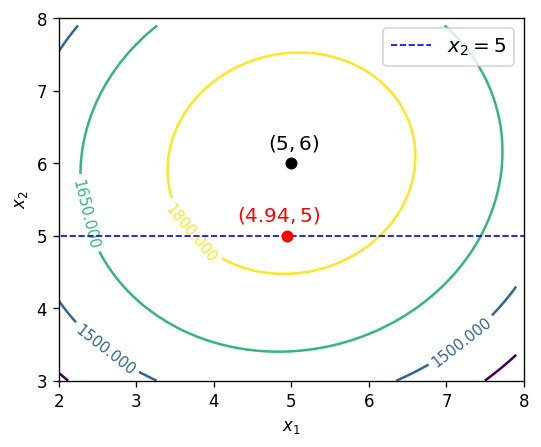
\includegraphics[width=0.45\textwidth]{lagrange}
	\caption{Решение задачи методом Лагранжа}
	\label{fig:lagrange}
\end{center}
\end{wrapfigure}

\newtheorem*{theorem1}{Критерий отрицательной определенности квадратичной формы}
\begin{theorem1}
Для отрицательной определенности квадратичной формы необходимо и достаточно, чтобы угловые миноры четного порядка ее матрицы были положительны, а нечетного порядка — отрицательны.
\end{theorem1}

Найдем главные миноры $H_L$:
\begin{center}
$\Delta_1 = \begin{vmatrix} -62 \end{vmatrix} = -62$\\
$\Delta_2 = \begin{vmatrix}
	-62 & 4 \\
	4 & -68
\end{vmatrix} = 4200$
\end{center}

По критерию отрицательной определенности квадратичной формы, матрица $H$ отрицательно определена. Таким образом, в соответствии с условиями второго порядка точка $(X^*, V^*)$ является точкой максимума $L(X, V)$ по $X$, а точка $X^* \approx (4.94, 5)$ -- решением задачи условной оптимизации, $f(X^*) \approx 1845$. 

\newpage

\section{Необходимые условия оптимальности при линейных ограничениях}

Запишем необходимые условия оптимальности Куна-Такера для задачи при ограничениях:
\begin{equation*}
\begin{cases}
	a_{11} x_1 + a_{12} x_2 \leq b_1 \\
	a_{21} x_1 + a_{22} x_2 \leq b_2 \\
	a_{31} x_1 + a_{32} x_2 \leq b_3 \\
	a_{41} x_1 + a_{42} x_2 \leq b_4 \\
\end{cases}
\Longleftrightarrow
\begin{cases}
	7 x_1 + 12 x_2 \leq 84 \\
	10 x_1 + 8 x_2 \leq 80 \\
	-x_1 \leq 0 \\
	-x_2 \leq 0
\end{cases}
\end{equation*}

\begin{equation*}
\begin{cases}
	\dfrac{\partial f}{\partial x_1} + u_1 \dfrac{\partial g_1}{\partial x_1} + u_2 \dfrac{\partial g_2}{\partial x_1} + u_3 \dfrac{\partial g_3}{\partial x_1} + u_4 \dfrac{\partial g_4}{\partial x_1} = 0 \\[0.3cm]
	\dfrac{\partial f}{\partial x_2} + u_1 \dfrac{\partial g_1}{\partial x_2} + u_2 \dfrac{\partial g_2}{\partial x_2} + u_3 \dfrac{\partial g_3}{\partial x_2} + u_4 \dfrac{\partial g_4}{\partial x_2} = 0 \\
	u_i g_i = 0, i = \overline{1,4} \\
	u_i \leq 0, i = \overline{1,4}
\end{cases}
\end{equation*}
\begin{equation*}
\begin{cases}
	-62 x_1 + 4 x_2 + 286 + 7 u_1 + 10 u_2 - u_3 = 0 \\
	-68 x_2 + 4 x_1 + 388 + 12 u_1 + 8 u_2 - u_4 = 0 \\
	u_1 (7 x_1 + 12 x_2 - 84) = 0 \\
	u_2 (10 x_1 + 8 x_2) = 0 \\
	u_3 x_1 = 0 \\
	u_4 x_2 = 0 \\
	u_i \leq 0, i = \overline{1,4}
\end{cases}
\end{equation*}

\section{Решение методом Била}

Запишем ограничения в канонической форме:
\begin{equation*}
\begin{cases}
	a_{11} x_1 + a_{12} x_2 \leq b_1 \\
	a_{21} x_1 + a_{22} x_2 \leq b_2 \\
	a_{31} x_1 + a_{32} x_2 \leq b_3 \\
	a_{41} x_1 + a_{42} x_2 \leq b_4 \\
\end{cases}
\Longleftrightarrow
\begin{cases}
	7 x_1 + 12 x_2 \leq 84 \\
	10 x_1 + 8 x_2 \leq 80 \\
	-x_1 \leq 0 \\
	-x_2 \leq 0
\end{cases}
\Longleftrightarrow
\begin{cases}
	7 x_1 + 12 x_2 + x_3 = 84 \\
	10 x_1 + 8 x_2 + x_4 = 80 \\
	x_i \geq 0, i = \overline{1,4}
\end{cases}
\end{equation*}

Найдем частные производные:

\begin{equation*}
	\begin{cases}
	\dfrac{\partial f}{\partial x_1} = -62 x_1 + 4 x_2 + 286 \\[0.3cm]
	\dfrac{\partial f}{\partial x_2} = -68 x_2 + 4 x_1 + 388
	\end{cases}
\end{equation*}

Пусть $\text{Б}_0 = \begin{pmatrix} 3 & 4 \end{pmatrix}$, тогда $X^{(0)} = \begin{pmatrix} 0 & 0 & 84 & 80 \end{pmatrix}^T$. Заполним симплекс-таблицу для опорной точки $X^{(0)}$, записав в последнюю строку формулы для частных производных:

\begin{table}[H]
\begin{center}
	\def\tabcolsep{15pt}
	\def\arraystretch{1.3}
	\caption{Базис $x_3, x_4$}
	\begin{tabular}{|c||c|c||c|}
		\hline
		$X^{(0)}$ & $x_1$ & $x_2$ & $b$ \\ 
		\hhline{|=#==#=|}
		$x_3$ & $-7$ & $-12$ & $84$ \\ 
		\hline
		$x_4$ & $-10$ & $-8$ & $80$ \\ 
		\hhline{|=#==#=|}
		$\sfrac{\partial f}{\partial x_j, u_j}$ & $-62 x_1 + 4 x_2 + 286$ & $-68 x_2 + 4 x_1 + 388$ &  \\ 
		\hline
	\end{tabular}
\end{center}
\end{table}

Базис является допустимым, так как $b \geq 0$, но не является оптимальным, так как $c = \begin{pmatrix} 286 & 388 \end{pmatrix} \nleqslant 0$.

Выберем как разрешающий столбец переменную $x_k	$, соответствующую максимальному значению производной целевой функции в точке $X^{(0)}$: 

$k = \argmax\limits_i\left\{\dfrac{\partial f}{\partial x_i}\left(X^{(0)}\right)\right\} = 2 \Rightarrow x_2$.

Оценим ситуацию в опорной точке $X^{(0)}$. Найдем соотношения между приращениями свободной переменной $x_2$ и изменениями базисных переменных $x_3$ и $x_4$ и частной производной по $x_2$:
\begin{itemize}
	\item $\dfrac{\partial f}{\partial x_2}\left(X^{(0)}\right) = 0$ при $x_2 \approx 5.7$
	\item $x_3 = 0$ при $x_2 = 7$
	\item $x_4 = 0$ при $x_2 = 10$
\end{itemize}

Производная обращается в ноль раньше базисных переменных, поэтому введем в задачу новую свободную переменную:
\begin{equation*}
	u_1 = \frac{1}{4} \cdot \frac{\partial f}{\partial x_2} = x_1 - 17 x_2 + 97
	\Longleftrightarrow
	x_2 = \frac{1}{17} \left(x_1 - u_1 + 97\right)
\end{equation*}

Заполним промежуточную таблицу, содержащую строку для новой переменной $u_1$. На пересечении $u_1$ и $x_2$ находится разрешающий элемент $-68$. 
\begin{table}[H]
\begin{center}
	\def\tabcolsep{25pt}
	\def\arraystretch{1.3}
	\caption{Промежуточная таблица базиса $x_3$, $x_4$ и $u_1$}
	\begin{tabular}{|c||c|c||c|}
		\hline
		$X^{(0)} \to X^{(1)}$ & $x_1$ & $x_2$ & $b$ \\ 
		\hhline{|=#==#=|}
		$u_1$ & $1$ & \textcolor{red}{\boldmath$-17$} & $97$ \\ 
		\hline
		$x_3$ & $-7$ & $-12$ & $84$ \\ 
		\hline
		$x_4$ & $-10$ & $-8$ & $80$ \\ 
		\hline
	\end{tabular}
\end{center}
\end{table}

Произведем перерасчет в соответствии с правилом перерасчета симплекс-таблиц. 

\begin{table}[H]
\begin{center}
	\def\tabcolsep{25pt}
	\def\arraystretch{1.3}
	\caption{Промежуточная таблица базиса $x_2$, $x_3$ и $x_4$}
	\begin{tabular}{|c||c|c||c|}
		\hline
		$X^{(0)} \to X^{(1)}$ & $x_1$ & $u_1$ & $b$ \\ 
		\hhline{|=#==#=|}
		$x_2$ & $-1$ & \textcolor{red}{\boldmath$1$} & $-97$ \\ 
		\hline
		$x_3$ & $131$ & $-12$ & $-264$ \\ 
		\hline
		$x_4$ & $178$ & $-8$ & $-584$ \\ 
		\hline
	\end{tabular}
\end{center}
\end{table}

Поделим на разрешающий элемент $-17$, а также выразим целевую функцию через свободные переменные и найдем частные производные:
\begin{align*}
	f(u_1, x_1) &= -31 x_1^2 - \frac{2}{17} \left(x_1 - u_1 + 97\right)^2 + \frac{4 x_1}{17} \left(x_1 - u_1 + 97\right) + \\ 
	&+ 286 x_1 + \frac{388}{17} \left(x_1 - u_1 + 97\right)
\end{align*}

\begin{equation*}
\begin{cases}
	\dfrac{\partial f}{\partial u_1} = \dfrac{4}{17} \left(x_1 - u_1 + 97\right) - \dfrac{4 x_1}{17} - \dfrac{388}{17} = -\dfrac{4 u_1}{17} \\[0.5cm]
	\dfrac{\partial f}{\partial x_1} = -62 x_1 + \dfrac{4 x_1}{17} + 286 + \dfrac{388}{17} = -\dfrac{1050 x_1}{17} + \dfrac{5250}{17}
\end{cases}
\end{equation*}

\begin{table}[H]
\begin{center}
	\def\tabcolsep{25pt}
	\def\arraystretch{1.3}
	\caption{Базис $x_2$, $x_3$ и $x_4$}
	\label{tab:simplex_1}
	\begin{tabular}{|c||c|c||c|}
		\hline
		$X^{(1)}$ & $x_1$ & $u_1$ & $b$ \\ 
		\hhline{|=#==#=|}
		$x_2$ & $\sfrac{1}{17}$ & $\sfrac{-1}{17}$ & $\sfrac{97}{17}$ \\ 
		\hline
		$x_3$ & \textcolor{red}{\boldmath$\sfrac{-131}{17}$} & $\sfrac{12}{17}$ & $\sfrac{264}{17}$ \\ 
		\hline
		$x_4$ & $\sfrac{-178}{17}$ & $\sfrac{8}{17}$ & $\sfrac{584}{17}$ \\ 
		\hhline{|=#==#=|}
		$\sfrac{\partial f}{\partial x_j, u_j}$ & $\sfrac{-1050 x_1 + 5250}{17}$ & $\sfrac{-4 u_1}{17}$ &  \\ 
		\hline
	\end{tabular}
\end{center}
\end{table}

Базис является допустимым, так как $b \geq 0$, но не является оптимальным, так как $c = \begin{pmatrix} \sfrac{5250}{17} & 0 \end{pmatrix} \nleqslant 0$.

Выберем как разрешающий столбец переменную $x_k$ ($u_k$), соответствующую максимальному значению производной целевой функции в точке $X^{(1)}$: 

$k = \argmax\limits_i\left\{\dfrac{\partial f}{\partial x_i}\left(X^{(1)}\right)\right\} = 1 \Rightarrow x_1$.

Оценим ситуацию в опорной точке $X^{(1)}$. Найдем соотношения между приращениями свободной переменной $x_1$ и изменениями базисных переменных $x_2$, $x_3$ и $x_4$ и частной производной по $x_1$:
\begin{itemize}
	\item $\dfrac{\partial f}{\partial x_1}\left(X^{(1)}\right) = 0$ при $x_1 = 5$
	\item $x_2 = 0$ при $x_1 = 98$
	\item $x_3 = 0$ при $x_1 \approx 1.9237$
	\item $x_4 = 0$ при $x_1 \approx -3.2359$
\end{itemize}

Переменная $x_3$ обращается в ноль раньше всех, поэтому выберем ее как разрешающую строку и произведем перерасчет симплекс-таблицы.

\begin{table}[H]
\begin{center}
	\def\tabcolsep{25pt}
	\def\arraystretch{1.3}
	\caption{Промежуточная таблица базиса $x_2$, $x_3$ и $x_4$}
	\label{tab:simplex_1}
	\begin{tabular}{|c||c|c||c|}
		\hline
		$X^{(1)} \to X^{(2)}$ & $x_3$ & $u_1$ & $b$ \\ 
		\hhline{|=#==#=|}
		$x_2$ & $\sfrac{1}{17}$ & $\sfrac{119}{17}$ & $\sfrac{-12971}{289}$ \\ 
		\hline
		$x_1$ & \textcolor{red}{\boldmath$1$} & $\sfrac{-12}{17}$ & $\sfrac{-264}{17}$ \\ 
		\hline
		$x_4$ & $\sfrac{-178}{17}$ & $\sfrac{-1088}{289}$ & $\sfrac{-74368}{289}$ \\ 
		\hline
	\end{tabular}
\end{center}
\end{table}

Поделим на разрешающий элемент $-17$, а также выразим целевую функцию через свободные переменные и найдем частные производные:
\begin{align*}
x_1 &= 84 - 12 x_2 - x_3,\ x_2 = \frac{1}{17} (x_1 - u_1 + 97) \\
17 x_2 &= 84 - 12 x_2 - x_3 - u_1 + 97 \Rightarrow 
x_2 = \frac{1}{29} (181 - x_3 - u_1) \\
x_1 &= 84 - \frac{1}{29} (2172 + 12 x_3 + 12 u_1) - x_3 = 
\frac{1}{29} (264 - 17 x_3 + 12 u_1)
\end{align*}

\begin{align*}
	f(u_1, x_3) &= -\frac{31}{841} (264 - 17 x_3 + 12 u_1)^2 - \frac{34}{841} (181 - x_3 - u_1)^2 + \\ 
	&+ \frac{4}{841} (264 - 17 x_3 + 12 u_1) (181 - x_3 - u_1) + \\ 
	&+ 286 (264 - 17 x_3 + 12 u_1) + 388 (181 - x_3 - u_1)
\end{align*}

\begin{equation*}
\begin{cases}
	\dfrac{\partial f}{\partial u_1} = \dfrac{4}{841} (2191 u_1 - 3174 x_3 + 6940) \\[0.5cm] % should be 694090
	\dfrac{\partial f}{\partial x_3} = -\dfrac{2}{841} (6348 u_1 - 8993 x_3 + 23472) % should be 2347281
\end{cases}
\end{equation*}

\begin{table}[H]
\begin{center}
	\def\tabcolsep{10pt}
	\def\arraystretch{1.3}
	\caption{Базис $x_1$, $x_2$ и $x_4$}
	\label{tab:simplex_1}
	\begin{tabular}{|c||c|c||c|}
		\hline
		$X^{(2)}$ & $x_3$ & $u_1$ & $b$ \\ 
		\hhline{|=#==#=|}
		$x_2$ & $\sfrac{-1}{131}$ & $\sfrac{-119}{131}$ & $\sfrac{12971}{2227}$ \\ 
		\hline
		$x_1$ & $\sfrac{-17}{131}$ & $\sfrac{12}{131}$ & $\sfrac{264}{131}$ \\ 
		\hline
		$x_4$ & $\sfrac{178}{131}$ & $\sfrac{1088}{2227}$ & $\sfrac{74368}{2227}$ \\ 
		\hhline{|=#==#=|}
		$\sfrac{\partial f}{\partial x_j, u_j}$ & $\sfrac{-2 (6348 u_1 - 8993 x_3 + 23472)}{841}$ & $\sfrac{4 (2191 u_1 - 3174 x_3 + 6940)}{841} $ &  \\ 
		\hline
	\end{tabular}
\end{center}
\end{table}

Базис является допустимым, так как $b \geq 0$, но не является оптимальным, так как $c = \begin{pmatrix} \sfrac{-4694562}{841} & \sfrac{2776360}{841} \end{pmatrix} \nleqslant 0$.

Выберем как разрешающий столбец переменную $x_k$ ($u_k$), соответствующую максимальному значению производной целевой функции в точке $X^{(1)}$: 

$k = \argmax\limits_i\left\{\dfrac{\partial f}{\partial x_i}\left(X^{(1)}\right)\right\} = 1 \Rightarrow u_1$.

Оценим ситуацию в опорной точке $X^{(2)}$. Найдем соотношения между приращениями свободной переменной $u_1$ и изменениями базисных переменных $x_1$, $x_2$ и $x_4$ и частной производной по $u_1$:
\begin{itemize}
	\item $\dfrac{\partial f}{\partial u_1}\left(X^{(2)}\right) = 0$ при $u_1 \approx 3.1679$
	\item $x_1 = 0$ при $u_1 \approx 23$
	\item $x_2 = 0$ при $u_1 \approx -6.4$
	\item $x_4 = 0$ при $u_1 \approx 65$
\end{itemize}

Производная обращается в ноль раньше базисных переменных, поэтому введем в задачу новую свободную переменную:
\begin{equation*}
	u_2 = \frac{1}{4} \cdot \frac{\partial f}{\partial u_1} = \frac{1}{841} (2191 u_1 - 3174 x_3 + 6940)
%	\Longleftrightarrow
%	u_1 = \frac{1}{2191} (841 u_2 + 3174 x_3 - 6940)
\end{equation*}

Заполним промежуточную таблицу, содержащую строку для новой переменной $u_1$. На пересечении $u_1$ и $u_2$ находится разрешающий элемент $\sfrac{2191}{841}$. 
\begin{table}[H]
\begin{center}
	\def\tabcolsep{25pt}
	\def\arraystretch{1.3}
	\caption{Промежуточная таблица базиса $x_1$, $x_2$, $x_4$ и $u_2$}
	\begin{tabular}{|c||c|c||c|}
		\hline
		$X^{(2)} \to X^{(3)}$ & $x_3$ & $u_1$ & $b$ \\ 
		\hhline{|=#==#=|}
		$x_2$ & $\sfrac{-1}{131}$ & $\sfrac{-119}{131}$ & $\sfrac{12971}{2227}$ \\ 
		\hline
		$x_1$ & $\sfrac{-17}{131}$ & $\sfrac{12}{131}$ & $\sfrac{264}{131}$ \\ 
		\hline
		$x_4$ & $\sfrac{178}{131}$ & $\sfrac{1088}{2227}$ & $\sfrac{74368}{2227}$ \\ 
		\hline
		$u_2$ & $\sfrac{3174}{841}$ & \textcolor{red}{\boldmath$\sfrac{2191}{841}$} & $\sfrac{-6940}{841}$ \\ 
		\hline
	\end{tabular}
\end{center}
\end{table}

Пересчитаем симплекс таблицу

\begin{table}[H]
\begin{center}
	\def\tabcolsep{17pt}
	\def\arraystretch{1.3}
	\caption{Промежуточная таблица базиса $x_1$, $x_2$, $x_4$ и $u_1$}
	\begin{tabular}{|c||c|c||c|}
		\hline
		$X^{(2)} \to X^{(3)}$ & $x_3$ & $u_2$ & $b$ \\ 
		\hhline{|=#==#=|}
		$x_2$ & $\sfrac{-379897}{110171}$ & $\sfrac{-119}{131}$ & $\sfrac{845873}{110171}$ \\ 
		\hline
		$x_1$ & $\sfrac{1}{131}$ & $\sfrac{12}{131}$ & $\sfrac{661704}{110171}$ \\ 
		\hline
		$x_4$ & $\sfrac{186862}{110171}$ & $\sfrac{1088}{2227}$ & $\sfrac{155389568}{1872907}$ \\ 
		\hline
		$u_1$ & $\sfrac{-3174}{841}$ & \textcolor{red}{\boldmath$1$} & $\sfrac{6940}{841}$ \\ 
		\hline
	\end{tabular}
\end{center}
\end{table}

Поделим каждый элемент промежуточной таблицы на разрешающий элемент и выразим целевую функцию через $u_2$ и $x_3$. 
\begin{align*}
	f(u_2, x_3) &= \dfrac{1}{2227} (82746 u_2 x_3 - 80030 u_2 - 4268 x_3^2 - 107230 x_3 - 8929)
\end{align*}

Дополним таблицу строкой, содержащей частные производные целевой функции по свободным переменным.
\vspace{-0.5cm}
\begin{table}[H]
\begin{center}
	\def\tabcolsep{10pt}
	\def\arraystretch{1.3}
	\caption{Базис $x_1$, $x_2$, $x_4$ и $u_1$}
	\begin{tabular}{|c||c|c||c|}
		\hline
		$X^{(3)}$ & $x_3$ & $u_2$ & $b$ \\ 
		\hhline{|=#==#=|}
		$x_2$ & $\sfrac{-379897}{110171}$ & $\sfrac{-119}{131}$ & $\sfrac{509045}{110171}$ \\ 
		\hline
		$x_1$ & $\sfrac{1}{131}$ & $\sfrac{12}{131}$ & $\sfrac{447691}{110171}$ \\ 
		\hline
		$x_4$ & $\sfrac{186862}{110171}$ & $\sfrac{1088}{2227}$ & $\sfrac{155389568}{1872907}$ \\ 
		\hline
		$u_1$ & $\sfrac{-3174}{841}$ & $\sfrac{841}{2227}$ & $\sfrac{6940}{841}$ \\ 
		\hhline{|=#==#=|}
		$\sfrac{\partial f}{\partial x_j, u_j}$ & $\sfrac{82746 u_2 - 8536 x_3 - 107230}{2227}$ & $\sfrac{82746 x_3 - 80030}{2227} $ &  \\ 
		\hline
	\end{tabular}
\end{center}
\end{table}

Базис является допустимым, так как $b \geq 0$, и является оптимальным, так как $c = \begin{pmatrix} \sfrac{-107230}{2227} & \sfrac{-80030}{2227} \end{pmatrix} \leq 0$. Следовательно оптимальным решением при заданных ограничениях является точка $X^{(3)} = \begin{pmatrix} 4.0636 & 4.6205 \end{pmatrix}^T$.

На рис. \ref{fig:bil} изображены траектория поиска точки максимума методом проекции градиента.
\vspace{-0.5cm}
\begin{figure}[H]
\begin{center}
	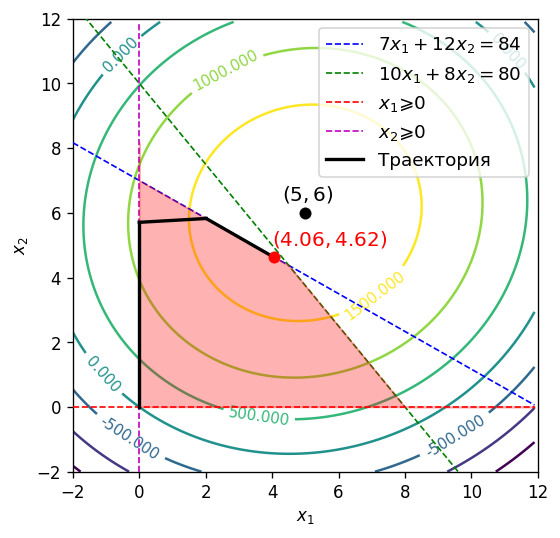
\includegraphics[width=0.7\textwidth]{bil}
	\caption{Траектория поиска методом Била}
	\label{fig:bil}
\end{center}
\end{figure}

\section{Решение методом проекции градиента}

Решим задачу при ограничениях:
\begin{equation*}
\begin{cases}
	a_{11} x_1 + a_{12} x_2 \leq b_1 \\
	a_{21} x_1 + a_{22} x_2 \leq b_2 \\
	a_{31} x_1 + a_{32} x_2 \leq b_3 \\
	a_{41} x_1 + a_{42} x_2 \leq b_4 \\
\end{cases}
\Longleftrightarrow
\begin{cases}
	7 x_1 + 12 x_2 \leq 84 \\
	10 x_1 + 8 x_2 \leq 80 \\
	-x_1 \leq 0 \\
	-x_2 \leq 0 \\
\end{cases}
\end{equation*}

Пусть $X^{(0)} = \begin{pmatrix} 0 & 0 \end{pmatrix}$. Запишем в матричной форме $A$, $b$ и $X$:
\begin{equation*}
A = \begin{pmatrix} 
	7 & 12 \\
	10 & 8 \\
	-1 & 0 \\
	0 & -1
\end{pmatrix},\ 
b = \begin{pmatrix} 
	84 \\
	80 \\
	0 \\
	0
\end{pmatrix}, \ 
X = \begin{pmatrix}
	x_1 \\
	x_2
\end{pmatrix}
\end{equation*}

Определим градиент $f'(X)$ и матрицу Гессе $H$ целевой функции:
\begin{equation*}
f'(X) = \begin{pmatrix} 
	-62 x_1 + 4 x_2 + 286 \\
	-68 x_2 + 4 x_1 + 388
\end{pmatrix}, 
H =
\begin{pmatrix}
	-62 & 4 \\
	4 & -68
\end{pmatrix}
\end{equation*}

Определим матрицы активных ограничений в точке $X^{(0)}$.

Убедимся в допустимости градиентного направления:
\begin{equation*}
A f'(X^{(0)}) = \begin{pmatrix}
	-1 & 0 \\
	0 & -1
\end{pmatrix} 
\cdot \begin{pmatrix}
	286 \\
	388
\end{pmatrix} =
 \begin{pmatrix}
	-286 \\
	-388
\end{pmatrix} < 0 
\end{equation*}

Следовательно
\begin{equation*}
K^{(0)} = f'(X^{(0)}) = \begin{pmatrix} 286 & 388 \end{pmatrix}^T
\end{equation*}

Выберем длину шага $t^{(0)}$.

Найдем множество нарушаемых ограничений $I_{pred}$:
\begin{equation*}
A K^{(0)} = \begin{pmatrix}
	7 & 12 \\
	10 & 8 \\
	-1 & 0 \\
	0 & -1
\end{pmatrix} \cdot \begin{pmatrix}
	286 \\
	388
\end{pmatrix} = \begin{pmatrix}
	6658 \\
	5964 \\
	-286 \\
	-388
\end{pmatrix}
\Longrightarrow
I_{pred} = \{1, 2\}
\end{equation*}

Найдем $t^{(0)}$:
\begin{equation*}
t^* = - \dfrac{\left\langle f'(X^{(0)}), K^{(0)} \right\rangle}{\left\langle K^{(0)}, HK^{(0)} \right\rangle} = 
- \dfrac{\begin{pmatrix} 286 & 388 \end{pmatrix} \begin{pmatrix} 286 & 388 \end{pmatrix}^T}{\begin{pmatrix} 286 & 388 \end{pmatrix} \begin{pmatrix} -62 & 4 \\ 4 & -68 \end{pmatrix} \begin{pmatrix} 286 \\ 388 \end{pmatrix}} \approx 0.0161
\end{equation*}

\begin{equation*}
t_{pred_1} = \dfrac{b_1 - a_1 X^{(0)}}{a_1 K^{(0)}} = \dfrac{84 - \begin{pmatrix} 7 & 12 \end{pmatrix} \begin{pmatrix} 0 & 0 \end{pmatrix}^T}{\begin{pmatrix} 7 & 12 \end{pmatrix} \begin{pmatrix} 286 \\ 388 \end{pmatrix}} = \dfrac{84}{6658} \approx 0.0126
\end{equation*}

\begin{equation*}
t_{pred_2} = \dfrac{b_2 - a_2 X^{(0)}}{a_2 K^{(0)}} = \dfrac{80 - \begin{pmatrix} 10 & 8 \end{pmatrix} \begin{pmatrix} 0 & 0 \end{pmatrix}^T}{\begin{pmatrix} 10 & 8 \end{pmatrix} \begin{pmatrix} 286 \\ 388 \end{pmatrix}} = \dfrac{80}{5964} \approx 0.0134
\end{equation*}

Следовательно $t^{(0)} = \min \left\{ t^*, t_{pred_1}, t_{pred_2} \right\} = 0.0126$.
 

\begin{equation*}
X^{(1)} = X^{(0)} + t^{(0)} K^{(0)} = \begin{pmatrix} 0 \\ 0 \end{pmatrix} + 0.0126 \begin{pmatrix} 286 \\ 388 \end{pmatrix} = \begin{pmatrix} 3.6036 \\ 4.8888 \end{pmatrix}
\end{equation*}

Сформируем матрицу активны ограничений.

Определим оператор проекции и направление $K^{(1)}$.

\begin{equation*}
A = \begin{pmatrix} 7 & 12 \end{pmatrix},\ 
f'(X^{(1)}) = \begin{pmatrix} 82.132 & 69.976 \end{pmatrix}^T
\end{equation*}

\begin{equation*}
P = E - A^T \left(A A^T\right)^{-1} A = \begin{pmatrix} 1 & 0 \\ 0 & 1 \end{pmatrix} - \begin{pmatrix} 0.2539 & 0.4352 \\ 0.4352 & 0.7461 \end{pmatrix} = \begin{pmatrix} 0.7461 & 0.4352 \\ -0.4352 & 0.2539 \end{pmatrix}
\end{equation*}

\begin{equation*}
K^{(1)} = P f'(X^{(1)}) = \begin{pmatrix} 0.7461 & 0.4352 \\ -0.4352 & 0.2539 \end{pmatrix} \begin{pmatrix} 82.132 \\ 69.976 \end{pmatrix} = \begin{pmatrix} 30.8251 \\ -17.9769 \end{pmatrix}
\end{equation*}

Найдем длину шага $t^{(1)}$.

Найдем множество нарушаемых ограничений $I_{pred}$:
\begin{equation*}
A K^{(1)} = \begin{pmatrix}
	7 & 12 \\
	10 & 8 \\
	-1 & 0 \\
	0 & -1
\end{pmatrix} \begin{pmatrix}
	30.8251 \\ 
	-17.9769
\end{pmatrix} = \begin{pmatrix}
	0 \\
	164.3944 \\
	-30.824 \\
	17.9806
\end{pmatrix}
\Longrightarrow
I_{pred} = \{2, 4\}
\end{equation*}

Найдем $t^{(1)}$:
\vspace{-0.9cm}
\begin{equation*}
t^* = - \dfrac{\left\langle f'(X^{(1)}), K^{(1)} \right\rangle}{\left\langle K^{(1)}, HK^{(1)} \right\rangle} \approx 0.0149
\end{equation*}
\begin{equation*}
t_{pred_2} = \dfrac{b_1 - a_1 X^{(1)}}{a_1 K^{(1)}} \approx 0.9437,\ \ 
t_{pred_4} = \dfrac{b_2 - a_2 X^{(1)}}{a_2 K^{(1)}} \approx 0.2718
\end{equation*}

Следовательно $t^{(1)} = \min \left\{ t^*, t_{pred_2}, t_{pred_4} \right\} = 0.0149$.
\begin{equation*}
X^{(2)} = X^{(1)} + t^{(1)} K^{(1)} = \begin{pmatrix} 3.6036 \\ 4.8888 \end{pmatrix} + 0.0149 \begin{pmatrix} 30.8251 \\ -17.9769 \end{pmatrix} = \begin{pmatrix} 4.0636 \\ 4.6205 \end{pmatrix}
\end{equation*}
Проверим условия останова:
\begin{equation*}
f'(X^{(2)}) = \begin{pmatrix} 52.5372 \\ 90.0637 \end{pmatrix}
\end{equation*}
\begin{equation*}
K^{(1)} = P f'(X^{(1)}) = \begin{pmatrix} 0.7461 & 0.4352 \\ -0.4352 & 0.2539 \end{pmatrix} \begin{pmatrix} 52.5372 \\ 90.0637 \end{pmatrix} = \begin{pmatrix} 0 \\ 0 \end{pmatrix}
\end{equation*}
\begin{equation*}
\Lambda = -\left(A A^T\right)^{-1} A f'(X^{(2)}) =
-\left( \begin{pmatrix} 7 & 12 \end{pmatrix} \begin{pmatrix} 7 \\ 12 \end{pmatrix}\right)^{-1} \begin{pmatrix} 7 & 12 \end{pmatrix} \begin{pmatrix} 52.5372 \\ 90.0637 \end{pmatrix} = -7.5053
\end{equation*}

$\Lambda \leq 0 \Rightarrow$ точка $X^{(2)} = \begin{pmatrix} 4.0636 & 4.6205 \end{pmatrix}^T$ является оптимальным решением задачи при заданных ограничениях. Значение целевой функции равно $f(X^{(2)}) \approx 1792$.

%На рис. \ref{fig:gradient} изображены траектория поиска точки максимума методом проекции градиента.
%\begin{figure}[H]
%\begin{center}
%	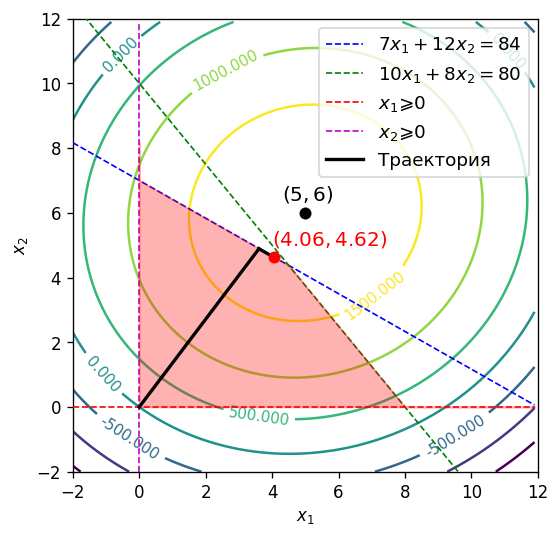
\includegraphics[width=0.8\textwidth]{gradient}
%	\caption{Траектория поиска методом проекции градиента}
%	\label{fig:gradient}
%\end{center}
%\end{figure}

На рис. \ref{fig:gradient} изображена траектория поиска оптимального решения при заданных ограничениях методом проекции градиента.
\vspace{-0.5cm}
\begin{figure}[H]
\begin{center}
	\begin{subfigure}[b]{0.49\textwidth}
		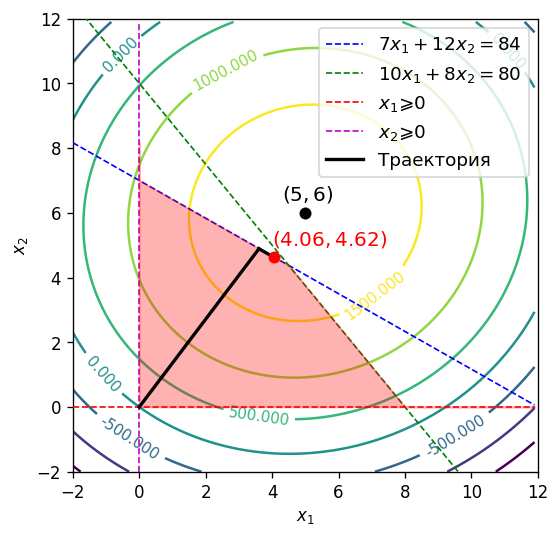
\includegraphics[width=1.03\textwidth]{gradient}
	\end{subfigure}
	\begin{subfigure}[b]{0.49\textwidth}
		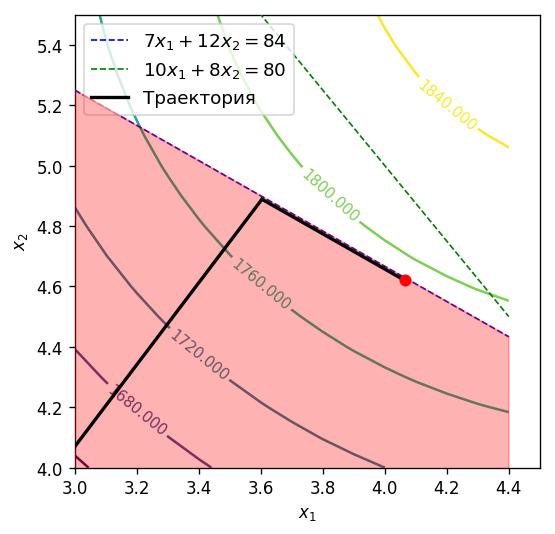
\includegraphics[width=1.02\textwidth]{gradient_zoom}
	\end{subfigure}
	\caption{Решение задачи методом проекции градиента}
	\label{fig:gradient}
\end{center}
\end{figure}

\section{Необходимые условия оптимальности при квадратичных ограничениях}

Запишем необходимые условия оптимальности Куна-Такера для задачи при ограничениях:
\begin{equation*}
d_1 x_1^2 + d_2 x_2^2 \leq b_6
\Longleftrightarrow
16 x_1^2 + 25 x_2^2 \leq 400
\end{equation*}
\begin{equation*}
\begin{cases}
	\dfrac{\partial f}{\partial x_1} + u_1 \dfrac{\partial g_1}{\partial x_1}  = 0 \\[0.3cm]
	\dfrac{\partial f}{\partial x_2} + u_1 \dfrac{\partial g_1}{\partial x_2}  = 0 \\
	u_1 g_1 = 0 \\
	u_1 \leq 0,
\end{cases}
\end{equation*}
\begin{equation*}
\begin{cases}
	-62 x_1 + 4 x_2 + 286 + 32 x_1 u_1 = 0 \\[0.3cm]
	-68 x_2 + 4 x_1 + 388 + 59 x_2 u_2 = 0 \\
	u_1 g_1 = 0 \\
	u_1 \leq 0
\end{cases}
\end{equation*}

\section{Решение методом штрафных функций}

Решим задачу при ограничении:
\begin{equation*}
d_1 x_1^2 + d_2 x_2^2 \leq b_6
\Longleftrightarrow
16 x_1^2 + 25 x_2^2 \leq 400
\end{equation*}

Обозначим ограничение функцией $g(x)$:
\begin{equation*}
g(X) = 16 x_1^2 + 25 x_2^2 - 400
\end{equation*}

Заменим исходную задачу условной оптимизации эквивалентной ей задачей безусловной оптимизации. Для этого введем функцию штрафов $\psi(x)$ и штрафную функцию $F(x)$:
\begin{equation*}
\psi(x) = \max \left\{ 0, x \right\}
\end{equation*}
\begin{equation*}
F(X, \mu) = f(X) - \mu \psi(g(X))
\end{equation*}

В таблице \ref{tab:penalty} приведены значения, полученные при различных значениях коэффициента $\mu$.
\begin{table}[H]
\begin{center}
	\pgfplotstabletypeset[col sep=comma,
	    columns={mu, x1, x2, f},
	    column type/.add={|c|}{},
	    columns/mu/.style={sci, column name={$\mu$}},
	    columns/x1/.style={fixed, precision=3, zerofill, column name={$x_1$}},
	    columns/x2/.style={fixed, precision=3, zerofill, column name={$x_2$}},
	    columns/f/.style={fixed, precision=3, zerofill, column name={$f(X)$}},
	    every nth row={1}{before row=\hline},
	    every head row/.style={before row=\hline, after row=\hline, },
	    every last row/.style={after row=\hline}
	   ]{../data/penalty.csv}
	   \caption{Решение методом штрафных функций}
	   \label{tab:penalty}
\end{center}
\end{table}

На рис. \ref{fig:penalty} изображена траектория поиска оптимального решения при заданных ограничениях методом штрафных функций.
\vspace{-0.5cm}
\begin{figure}[H]
\begin{center}
	\begin{subfigure}[b]{0.49\textwidth}
		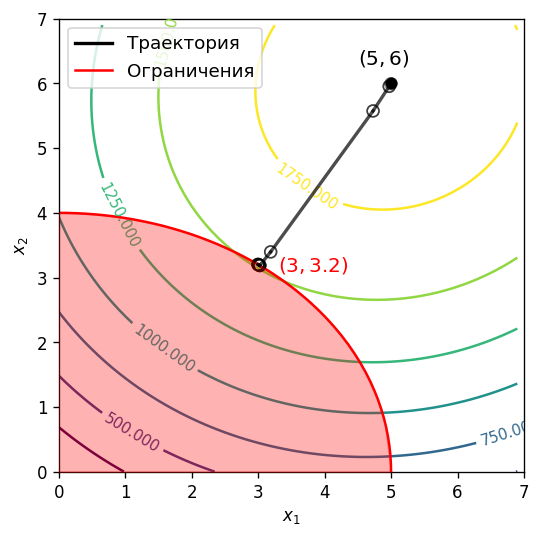
\includegraphics[width=\textwidth]{penalty}
	\end{subfigure}
	\begin{subfigure}[b]{0.49\textwidth}
		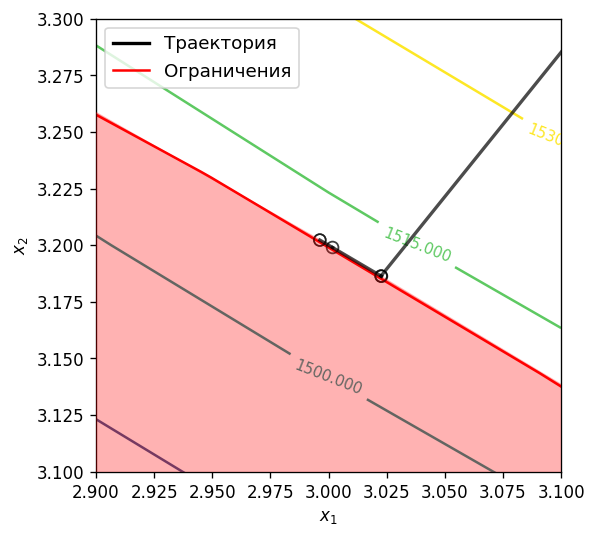
\includegraphics[width=1.1\textwidth]{penalty_zoom}
	\end{subfigure}
	\caption{Решение задачи методом штрафных функций}
	\label{fig:penalty}
\end{center}
\end{figure}

\newpage

\section{Решение методом возможных направлений}

Решим задачу при ограничении:
\begin{equation*}
d_1 x_1^2 + d_2 x_2^2 \leq b_6
\Longleftrightarrow
16 x_1^2 + 25 x_2^2 \leq 400
\end{equation*}

При поиске на границе области формулируется вспомогательная задача линейного программирования:
\begin{equation*}
\begin{cases}
\max u \\
\left\langle f'(X^{(i)}, K^{(i)} \right\rangle \geq u \\
\left\langle g_l'(X^{(i)}, K^{(i)} \right\rangle \geq u, l \in I \\
u \geq 0
\end{cases}
\end{equation*}

В таблице \ref{tab:available} приведены значения, полученные на каждом шаге работы алгоритма.
\begin{table}[H]
\begin{center}
	\pgfplotstabletypeset[col sep=comma,
	    columns={i, x1, x2, u, f, k1, k2},
	    column type/.add={|c|}{},
	    columns/i/.style={fixed, column name={$i$}},
	    columns/x1/.style={fixed, precision=3, zerofill, column name={$x_1$}},
	    columns/x2/.style={fixed, precision=3, zerofill, column name={$x_2$}},
	    columns/u/.style={fixed, precision=3, zerofill, column name={$u$}},
	    columns/f/.style={fixed, precision=3, zerofill, column name={$f(X)$}},
	    columns/k1/.style={fixed, precision=3, zerofill, column name={$k_1$}},
	    columns/k2/.style={fixed, precision=3, zerofill, column name={$k_2$}},
	    every nth row={1}{before row=\hline},
	    every head row/.style={before row=\hline, after row=\hline, },
	    every last row/.style={after row=\hline}
	   ]{../data/available.csv}
	   \caption{Решение методом возможных направлений}
	   \label{tab:available}
\end{center}
\end{table}

На рис. \ref{fig:available} изображена траектория поиска оптимального решения при заданных ограничениях методом возможных направлений.
\vspace{-0.5cm}
\begin{figure}[H]
\begin{center}
	\begin{subfigure}[b]{0.49\textwidth}
		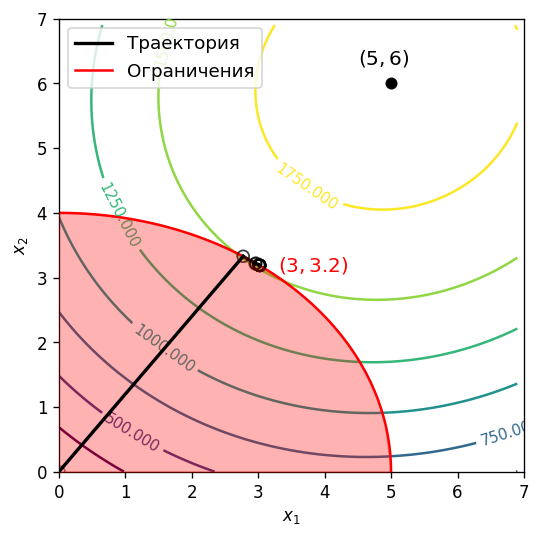
\includegraphics[width=\textwidth]{available}
	\end{subfigure}
	\begin{subfigure}[b]{0.49\textwidth}
		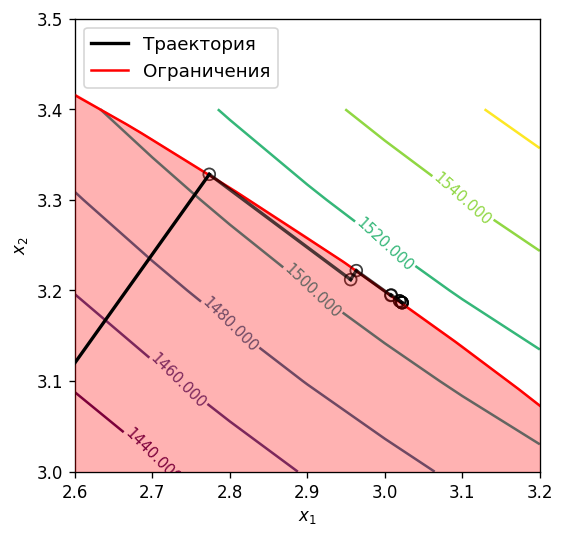
\includegraphics[width=1.04\textwidth]{available_zoom}
	\end{subfigure}
	\caption{Решение задачи методом возможных направлений}
	\label{fig:available}
\end{center}
\end{figure}

\end{document}